\input{preambolo_comune}

\title{Controllo degli Accessi}
\author{Basato sulle slide della Prof.ssa Jocelyne Elias}
\date{\today}

\begin{document}

\maketitle
\tableofcontents
\newpage

\section{Introduzione al Controllo degli Accessi}
Il controllo degli accessi è un meccanismo di sicurezza fondamentale che segue la fase di autenticazione. Una volta verificata l'identità di un utente (chi è), è necessario determinare quali azioni è autorizzato a compiere (cosa può fare).

\subsection{Obiettivi del Controllo degli Accessi}
Gli obiettivi principali sono:
\begin{itemize}
    \item Impedire agli utenti non autorizzati di accedere alle risorse.
    \item Impedire agli utenti legittimi di accedere alle risorse in modo non autorizzato (es. un utente può leggere un file ma non modificarlo).
    \item Permettere agli utenti legittimi di accedere alle risorse nel modo autorizzato.
\end{itemize}
Si basa su un insieme di \textbf{politiche} (regole) e \textbf{meccanismi} (strumenti tecnici) per decidere se un \textbf{soggetto} può eseguire determinate \textbf{operazioni} su specifici \textbf{oggetti}.

\subsection{Elementi Fondamentali}
\begin{description}
    \item[Soggetto (Subject)] L'entità che richiede l'accesso (es. utente, processo, script).
        \begin{itemize}
            \item \textit{Esempio pratico:} Utente \texttt{mario.rossi}, processo \texttt{excel.exe}.
        \end{itemize}
    \item[Oggetto (Object)] La risorsa da proteggere (es. file, database, stampante).
        \begin{itemize}
            \item \textit{Esempio pratico:} File \texttt{budget.xlsx}, tabella \texttt{Clienti}.
        \end{itemize}
    \item[Diritto di Accesso (Access Right)] Il tipo di interazione permessa tra soggetto e oggetto.
        \begin{itemize}
            \item \textit{Esempi comuni:} \texttt{read}, \texttt{write}, \texttt{execute}, \texttt{delete}, \texttt{own}.
        \end{itemize}
\end{description}

\section{Tipi di Politiche di Controllo degli Accessi}

\subsection{Discretionary Access Control (DAC)}
\begin{itemize}
    \item L'accesso si basa sull'identità del soggetto e su regole definite dal proprietario dell'oggetto.
    \item \textit{Discrezionale}: il proprietario decide chi può accedere e come.
    \item \textit{Esempio pratico:} Il creatore di un file decide di condividerlo in lettura con un collega.
\end{itemize}

\subsection{Mandatory Access Control (MAC)}
\begin{itemize}
    \item L'accesso si basa sul confronto tra etichette di sicurezza (oggetti) e autorizzazioni (soggetti).
    \item \textit{Obbligatorio}: le etichette e le autorizzazioni sono gestite centralmente dal sistema e non modificabili dai singoli utenti.
    \item \textit{Esempio pratico:} In ambito militare, un utente con nulla osta \texttt{RISERVATO} non può accedere a documenti \texttt{TOP SECRET}.
\end{itemize}

\subsection{Role-Based Access Control (RBAC)}
\begin{itemize}
    \item L'accesso si basa sui ruoli assegnati ai soggetti.
    \item I permessi sono associati ai ruoli, e gli utenti ereditano i permessi dei ruoli che ricoprono.
    \item \textit{Esempio pratico:} Un utente con ruolo \texttt{CONTABILE} ha accesso ai sistemi di contabilità, mentre un utente con ruolo \texttt{VENDITORE} accede al CRM.
\end{itemize}

\section{Principi Fondamentali per le Politiche di Sicurezza}
\begin{itemize}
    \item \textbf{Open Design:} La sicurezza non deve dipendere dalla segretezza del design del meccanismo.
    \item \textbf{Economy of Mechanism:} I meccanismi di sicurezza devono essere il più semplici possibile.
    \item \textbf{Fail-safe Defaults:} L'accesso deve essere negato di default e concesso solo esplicitamente.
    \item \textbf{Complete Mediation (Reference Monitor):} Ogni tentativo di accesso deve essere verificato. Il \textit{Reference Monitor} è il componente (astratto) che applica questa mediazione; deve essere inviolabile, sempre invocato e verificabile.
    \item \textbf{Least Privilege (Minimo Privilegio):} Ogni soggetto deve operare con il minor numero di privilegi necessari per svolgere il proprio compito.
        \begin{itemize}
            \item Limita i danni in caso di errore o compromissione.
            \item \textit{Esempio pratico:} Un server web necessita solo di leggere i file del sito e ascoltare su porte specifiche, non di modificare file di sistema.
        \end{itemize}
\end{itemize}

\section{Notazione Formale}
\begin{itemize}
    \item $S$: Insieme dei soggetti.
    \item $O$: Insieme degli oggetti.
    \item $\alpha$: Insieme dei diritti di accesso.
\end{itemize}

\section{Domini di Protezione}
\begin{itemize}
    \item Un dominio di protezione è un insieme di coppie $\langle oggetto, \text{insieme\_dei\_diritti\_di\_accesso} \rangle$.
    \item I soggetti operano all'interno di un dominio. L'associazione può essere \textbf{statica} o \textbf{dinamica}.
    \item \textit{Esempio (dinamica):} Modalità \texttt{Kernel mode} vs \texttt{User mode} nei sistemi operativi. Un processo in \texttt{user mode} passa temporaneamente in \texttt{kernel mode} (dominio con privilegi più alti) per eseguire una system call.
\end{itemize}

\section{Modello della Matrice di Controllo degli Accessi (ACM)}
Modello per DAC, con domini/soggetti come righe e oggetti come colonne. Ogni cella $M(i, j)$ contiene i diritti $\alpha$ del dominio $D_i$ sull'oggetto $O_j$.

\subsection{Esempio Base di ACM}
\begin{table}[H]
    \centering
    \caption{Esempio Base di Matrice di Controllo degli Accessi}
    \label{tab:acm_base}
    \begin{tabular}{|l|l|l|l|l|}
        \hline
        \rowcolor{black!80}\textbf{SOGGETTI / OGGETTI} & \textbf{File 1} & \textbf{File 2} & \textbf{File 3} & \textbf{File 4} \\ \hline
        \textbf{User A} & \texttt{Own,R,W} & & \texttt{Own,R,W} & \\ \hline
        \textbf{User B} & \texttt{R} & \texttt{Own,R,W} & \texttt{W} & \texttt{R} \\ \hline
        \textbf{User C} & \texttt{R,W} & \texttt{R} & & \texttt{Own,R,W} \\ \hline
    \end{tabular}
\end{table}

\subsection{Esempio Avanzato di ACM con Domini e Diritto \texttt{switch}}
Per implementare il principio del minimo privilegio, si possono usare domini specializzati e un diritto \texttt{switch} per passare da un dominio all'altro, copiando selettivamente i diritti necessari.

\begin{table}[H]
    \centering
    \caption{Matrice di Controllo Accessi con Meccanismo \texttt{switch} e Copia dei Diritti (basato su slide 15)}
    \label{tab:acm_switch_slide15}
    \begin{tabular}{|l|l|l|l|l|l|}
        \hline
        \rowcolor{black!80}\textbf{Dominio/Soggetto} & \textbf{File1} & \textbf{File2} & \textbf{File3} & \textbf{File4} & \textbf{D4 (dominio)} \\ \hline
        D1 (es. A)          & \texttt{read}  &                &                &               &                       \\ \hline
        A (in D2)           &                & \texttt{R,W}   & \texttt{R}     &               & \texttt{switch}       \\ \hline
        B (in D3)           &                &                & \texttt{R,W}   &               & \texttt{switch}       \\ \hline
        \multicolumn{6}{|l|}{\textit{Situazione dopo lo switch (istanze di D4 con diritti copiati):}} \\ \hline
        A (in istanza D4)   &                & \texttt{R,W}   & \texttt{R}     & \texttt{R}    &                       \\ \hline
        B (in istanza D4)   &                &                & \texttt{R,W}   & \texttt{R}    &                       \\ \hline
    \end{tabular}
     \parbox{\linewidth}{\footnotesize Il dominio D4 è specializzato (es. per accesso al dizionario File4). Quando A (da D2) e B (da D3) fanno \texttt{switch} a un'istanza di D4, mantengono i diritti sui file che stavano editando (File2, File3) e ottengono i diritti specifici di D4 (es. \texttt{read} su File4).}
\end{table}

\section{Implementazione della Matrice di Controllo degli Accessi}

\subsection{Tabella Globale}
\begin{itemize}
    \item Memorizza la matrice come array 2D.
    \item \textbf{Vantaggi:} Semplice.
    \item \textbf{Svantaggi:} Può essere enorme (matrici sparse), difficile da mantenere in sistemi dinamici.
\end{itemize}

\subsection{Access Control Lists (ACLs)}
\begin{itemize}
    \item Matrice memorizzata "per colonna": ad ogni \textbf{oggetto} è associata una lista di $\langle \text{dominio/soggetto, diritti} \rangle$.
    \item \textit{Analogia:} Lista degli invitati a una festa.
    \item \textit{Esempio (UNIX):} Il comando \texttt{ls -l} mostra una forma di ACL.
    \begin{minted}{bash}
babaoglu% ls -l /etc/passwd
-rw-r--r-- 1 root wheel 7579 Jan 1 2020 /etc/passwd
    \end{minted}
    UNIX ha 3 "domini" per file: \texttt{owner} (proprietario), \texttt{group} (gruppo), \texttt{others} (altri).
    \item \textit{Diagramma ACL (esempio concettuale):}
    \begin{itemize}
        \item \textbf{File 1} $\rightarrow$ [ (User A: \texttt{Own,R,W}), (User B: \texttt{R}), (User C: \texttt{R,W}) ]
        \item \textbf{File 2} $\rightarrow$ [ (User B: \texttt{Own,R,W}), (User C: \texttt{R}) ]
    \end{itemize}
\end{itemize}

\subsection{Capabilities (Capacità)}
\begin{itemize}
    \item Matrice memorizzata "per riga": ad ogni \textbf{soggetto} è associata una lista di $\langle \text{oggetto, diritti} \rangle$. Ogni tupla è una capability.
    \item \textit{Analogia:} Una chiave per una serratura o un invito per una festa.
    \item Il soggetto presenta la capability per accedere.
    \item \textit{Diagramma Capability (esempio concettuale):}
    \begin{itemize}
        \item \textbf{User A} $\rightarrow$ [ (File 1: \texttt{Own,R,W}), (File 3: \texttt{Own,R,W}) ]
        \item \textbf{User B} $\rightarrow$ [ (File 1: \texttt{R}), (File 2: \texttt{Own,R,W}), (File 3: \texttt{W}) ]
    \end{itemize}
    \item \textbf{Garanzie necessarie:}
    \begin{enumerate}
        \item Le capability non devono essere falsificabili.
        \item L'oggetto (o reference monitor) deve poterle verificare.
        \item La copia/trasferimento deve essere controllata.
    \end{enumerate}
    \item \textbf{Implementazione con crittografia a chiave pubblica:}
    Una capability $\langle \text{oggetto, diritti, codice\_unico} \rangle$ viene firmata digitalmente con la chiave privata dell'oggetto. Il processo non può modificarla senza invalidare la firma.
\end{itemize}

\section{Revoca dei Diritti di Accesso}
La revoca può essere immediata/ritardata, selettiva/generale, parziale/totale, temporanea/permanente.
\begin{itemize}
    \item \textbf{Sistemi ACL-based:} Facile, si modifica l'ACL dell'oggetto.
    \item \textbf{Sistemi Capability-based:} Difficile, le capability sono distribuite. Soluzioni:
    \begin{itemize}
        \item \textbf{Capability a tempo limitato:} Scadono e necessitano rinnovo (revoca ritardata).
        \item \textbf{Capability Indirette:} Puntano a tabelle intermedie; modificando la tabella si revoca l'accesso (revoca immediata).
    \end{itemize}
\end{itemize}

\section{Esempio: Controllo Accessi nel File System UNIX}
UNIX utilizza un modello ibrido.

\subsection{Oggetti, Struttura e Permessi Base}
\begin{itemize}
    \item Ogni risorsa è un file in una struttura ad albero.
\begin{figure}[H]
\centering
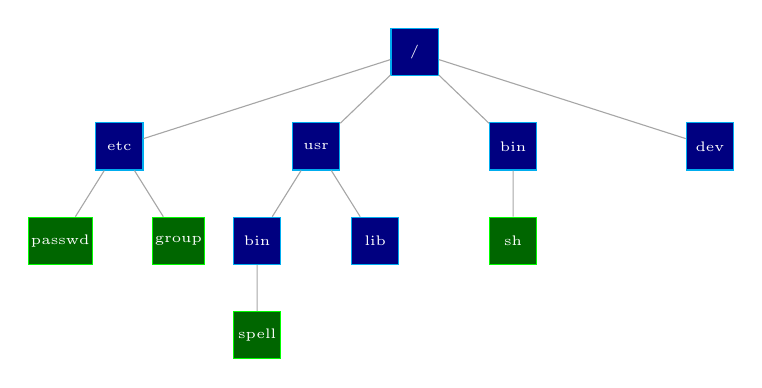
\begin{tikzpicture}[
    level 1/.style={sibling distance=25mm, level distance=12mm},
    level 2/.style={sibling distance=15mm, level distance=12mm},
    level 3/.style={sibling distance=10mm, level distance=12mm},
    dir/.style={rectangle, draw=cyan, fill=blue!50!black, text=white, minimum size=6mm, font=\tiny, inner sep=1pt},
    file/.style={rectangle, draw=green, fill=green!40!black, text=white, minimum size=6mm, font=\tiny, inner sep=1pt},
    tree_link/.style={draw=gray!70} % Stile per i collegamenti dell'albero
]
\node[dir] (root) {/}
    child[tree_link] {node[dir] (etc) {etc}
        child[tree_link] {node[file] (passwd) {passwd}}
        child[tree_link] {node[file] {group}}
    }
    child[tree_link] {node[dir] (usr) {usr}
        child[tree_link] {node[dir] (bin_usr) {bin}
            child[tree_link] {node[file] (spell) {spell}}
        }
        child[tree_link] {node[dir] (lib_usr) {lib}}
    }
    child[tree_link] {node[dir] (bin) {bin}
        child[tree_link] {node[file] (sh) {sh}}
    }
    child[tree_link] {node[dir] (dev) {dev}};
\end{tikzpicture}
\caption{Struttura ad albero semplificata del file system UNIX.}
\label{fig:unix_fs_tree}
\end{figure}
    \item Ogni file ha un \texttt{owner} e un \texttt{group}.
    \item 9 bit di permessi: 3 per \texttt{owner} (\texttt{rwx}), 3 per \texttt{group} (\texttt{rwx}), 3 per \texttt{others} (\texttt{rwx}).
    \begin{itemize}
        \item \texttt{rw-r--r--} (ottale 644)
        \item \texttt{rwxr-xr-x} (ottale 755)
    \end{itemize}
    \item User e group ID sono interi (da \texttt{/etc/passwd}). Esempio di riga in \texttt{/etc/passwd}:
    \begin{minted}{text}
mezzina:x:501:1000:Leonardo Mezzina:/home/mezzina:
trotter:x:502:1000:Guido Trotter:/home/trotter:
    \end{minted}
    Qui \texttt{501} è user-id, \texttt{1000} è group-id per \texttt{mezzina}.
\end{itemize}

\subsection{ID dei Processi: Reali vs Effettivi}
Ogni processo ha:
\begin{itemize}
    \item \textbf{\texttt{real-user-id} (RUID), \texttt{real-group-id} (RGID):} Identificano l'utente che ha lanciato il processo. Non cambiano.
    \item \textbf{\texttt{effective-user-id} (EUID), \texttt{effective-group-id} (EGID):} Usati dal kernel per i controlli di accesso. Normalmente EUID=RUID. Possono cambiare (es. via \texttt{setuid}).
\end{itemize}

\subsection{Meccanismo Ibrido: \texttt{open()} e File Descriptors}
\begin{itemize}
    \item La system call \texttt{int open(const char *pathname, int flags);}
    \begin{minted}{c}
int open(const char *pathname, int flags); // flags: O_RDONLY, O_WRONLY, O_RDWR
    \end{minted}
    \item \texttt{open()} controlla i permessi del file rispetto a EUID/EGID del processo (controllo ACL-like).
    \item Se permesso, restituisce un \textbf{file descriptor (fd)}: un intero che è un indice nella \textit{File Descriptor Table} del processo.
    \item Ogni voce in questa tabella (associata a un fd) agisce come una \textbf{capability}: dà al processo il diritto di operare sul file (con \texttt{read()}, \texttt{write()}) \textbf{senza ulteriori controlli ACL}.
    \item Il costoso controllo ACL è fatto solo una volta (su \texttt{open()}).
\end{itemize}
\begin{figure}[H]
\centering
\begin{tikzpicture}[
    node distance=0.4cm and 0.8cm, % ridotta distanza orizzontale
    % Stili ereditati da quelli globali, ma posso sovrascriverli se necessario
]

% Process Descriptor Table (semplificato)
\node[proc] (process_table) {Process \\ Descriptor \\ Table};

% File Descriptor Table
\node[fdt, right=1.5cm of process_table] (file_desc_table) {File Descriptor Table};
\node[fdentry, at=(file_desc_table.north west), yshift=-0.15cm, xshift=0.1cm] (fd0) {0: STDIN};
\node[fdentry, below=0.05cm of fd0] (fd1) {1: STDOUT};
\node[fdentry, below=0.05cm of fd1] (fd2) {2: STDERR};
\node[fdentry, below=0.05cm of fd2] (fd3) {3: File};
\node[font=\Large, below=0.2cm of fd3, text=white, xshift=0.8cm] (dots) {\vdots};

% Hardware/File Objects
\node[obj, right=1cm of fd0] (stdin_obj) {Keyboard \\ File Object};
\node[hw, right=0.8cm of stdin_obj] (keyboard_hw) {Tastiera};
\path[fdlink] (stdin_obj.east) -- (keyboard_hw.west) node[midway, text=white, font=\Large] {$=$};

\node[obj, right=1cm of fd1, yshift=-0.2cm] (stdout_obj) {Monitor \\ File Object};
\node[hw, right=0.8cm of stdout_obj] (monitor_hw1) {Monitor};
\path[fdlink] (stdout_obj.east) -- (monitor_hw1.west) node[midway, text=white, font=\Large] {$=$};

% STDERR punta allo stesso monitor di STDOUT
\node[obj, right=1cm of fd2, yshift=0.1cm] (stderr_obj) {Monitor \\ File Object};
\path[fdlink] (stderr_obj.east) -| ($(monitor_hw1.west) + (-0.1,0)$) node[midway, text=white, font=\Large] {$=$};


\node[obj, below=0.3cm of stderr_obj, xshift=0cm, yshift=-0.1cm] (file_obj) {I/O \\ File Object}; % Posizionato per fd3
\node[hw, right=0.8cm of file_obj] (disk_hw) {Disco/File};
\path[fdlink] (file_obj.east) -- (disk_hw.west) node[midway, text=white, font=\Large] {$=$};


% Links da FDT entries to Objects
\draw[fdlink] (fd0.east) -- (stdin_obj.west);
\draw[fdlink] (fd1.east) -- (stdout_obj.west);
\draw[fdlink] (fd2.east) -- (stderr_obj.west);
\draw[fdlink] (fd3.east) -- (file_obj.west);

% Link da Process Table a FDT (simbolico)
\draw[fdlink] ($(process_table.east)+(0,0.3cm)$) .. controls +(0.2,0) and +(-0.2,0) .. ($(file_desc_table.west)+(0,0.3cm)$);
\draw[fdlink] ($(process_table.east)+(0,-0.3cm)$) .. controls +(0.2,0) and +(-0.2,0) .. ($(file_desc_table.west)+(0,-0.3cm)$);

\end{tikzpicture}
\caption{Tabella dei File Descriptor e oggetti associati in UNIX (modello ibrido).}
\label{fig:fd_table_unix}
\end{figure}

\subsection{\texttt{saved-user-id} (SUID)}
Ogni processo ha anche un \texttt{saved-user-id} (e \texttt{saved-group-id}) che memorizza l'EUID (o EGID) al momento dell'esecuzione di un programma \texttt{setuid}. Permette di ripristinare i privilegi originali.

\subsection{Meccanismo \texttt{set-user-id} (\texttt{setuid}) e \texttt{set-group-id} (\texttt{setgid})}
\begin{itemize}
    \item Se un file eseguibile ha il bit \texttt{setuid} impostato:
    \begin{itemize}
        \item Quando eseguito, il SUID del processo = EUID corrente.
        \item L'EUID del processo = user-id del \textbf{proprietario del file eseguibile}.
    \end{itemize}
    \item Permette a un utente di eseguire un programma con i permessi del proprietario del programma.
    \item I nuovi permessi (EUID elevato) valgono solo per la durata del programma \texttt{setuid}.
    \item Utile per implementare il \textit{principio del minimo privilegio}.
\end{itemize}

\subsection{Esempio di \texttt{setuid}: il comando \texttt{passwd}}
\begin{itemize}
    \item Problema: Permettere agli utenti di cambiare la propria password (in \texttt{/etc/passwd} o \texttt{/etc/shadow}, file di proprietà di \texttt{root}) senza dare loro accesso diretto al file.
    \item Soluzione:
    \begin{enumerate}
        \item File \texttt{/etc/passwd} (o \texttt{/etc/shadow}) è di \texttt{root}, permessi tipo \texttt{rw-------}.
        \begin{minted}{text}
# Esempio permessi /etc/shadow
-r-------- 1 root root ... /etc/shadow
        \end{minted}
        \item Programma \texttt{/bin/passwd} è di \texttt{root} e ha il bit \texttt{setuid} attivo.
        \begin{minted}{text}
# Esempio permessi /usr/bin/passwd
-r-s--x--x 1 root root ... /usr/bin/passwd
        \end{minted}
        (La \texttt{s} indica \texttt{setuid} e \texttt{execute} per l'owner).
        \item Quando un utente (es. \texttt{alice}) esegue \texttt{/bin/passwd}:
        \begin{itemize}
            \item RUID del processo = \texttt{alice}.
            \item EUID del processo = \texttt{root} (grazie al \texttt{setuid} e al fatto che \texttt{/bin/passwd} è di \texttt{root}).
            \item Il programma \texttt{/bin/passwd} (ora con EUID=\texttt{root}) può scrivere in \texttt{/etc/passwd}.
            \item Il programma stesso deve contenere logica per assicurare che \texttt{alice} (RUID) cambi solo la propria password.
        \end{itemize}
    \end{enumerate}
\end{itemize}
\begin{minted}{c}
// Pseudo-codice di un programma come passwd
int main() {
    uid_t ruid = getuid(); // Real User ID
    uid_t euid = geteuid(); // Effective User ID

    // Se euid == 0 (root), allora abbiamo privilegi elevati
    if (euid == 0) {
        // Verifica che l'utente ruid stia cambiando la propria password
        // Chiedi vecchia password, nuova password, etc.
        // Scrivi nel file delle password (es. /etc/shadow)
        
        // Opzionale: abbassa i privilegi se non più necessari
        // seteuid(ruid); 
    } else {
        // Non abbiamo privilegi di root
        printf("Errore: privilegi insufficienti.\n");
        return 1;
    }
    return 0;
}
\end{minted}

\end{document}